\chapter{Iterative development}\label{chapter:prototype}

% Shirley et al. : human-centered design process
%This iterative process can be human-centered design process described in \cite{shirley:2009}.

This chapter describes how the idea presented in chapter \ref{chapter:whitebox} is tested and improved through different development cycles. First the evaluation and development techniques used for the tests are described.


\section{Methodology}\label{chapter:prototype:section:methodology}

\subsection{Prototyping}\label{chapter:prototype:section:methodology:subsection:development}

% rapid prototyping

There are three types of prototypes that were used in the iterations:

\begin{itemize}
	\item Paper prototype;
	\item Digital prototype with 'fake' data or interaction effects;
	\item Digital prototype with working implementation.
\end{itemize}

It is obvious that for each category the resources that are required to build the prototype differ. The objective is to filter out most of the issues in the low cost designs, avoiding a greater cost in the more expensive prototypes.

% paper prototyping
%\subsubsection{Paper prototype}\label{chapter:prototype:s:methodology:ss:development:sss:paper}

\emph{Paper prototyping}\index{paper prototyping} is defined as "a variation of usability testing where representative users perform realistic tasks by interacting with a paper version of the interface that is manipulated by a person 'playing computer', who doesn’t explain how the interface is intended to work"\cite{snyder:2003:web}. It is a technique for designing, testing, and refining user interfaces \cite{snyder:2003}, and is closely related to usability testing \cite{snyder:2003:web}. In the last decade it has become a regularly applied technique in major businesses such as IBM, Digital, Honeywell, and Microsoft among others\cite{snyder:2003}.

%In \cite{usabilitynet:2006:paperprototyping} a number of benefits are associated with paper prototyping:
%\begin{itemize}
%	\item Usability problems can be already detected in the early stages of the design process, even before any code has been written.
%	\item The promotion of communication between designers and users.
%	\item Paper prototypes can be created and refined relatively easily, allowing for rapid design iterations.
%	\item Creating a paper prototype requires little resources.
%\end{itemize}


\subsection{Evaluation techniques}\label{chapter:prototype:section:methodology:subsection:evaluation}

The evaluation of an application prototype can be performed using one or more different techniques, and based on a range of varying criteria, such as: usability, usefulness, meaning, efficiency, accuracy and so on. Various techniques exist, such as questionnaires, usability engineering, expert evaluation, and usage tracking\cite{duval:2012:chi:evaluation}.

Methods may be \emph{formative}\index{formative!evaluation technique} or \emph{summative}\index{summative!evaluation technique}. Formative means that the evaluation occurs simultaneously with user task execution. Summative occurs after the user has performed all the required tasks\cite{duval:2012:chi:evaluation}.

The methods we will be using here are a variation on \emph{usability engineering}\index{usability engineering} called \emph{think aloud}\index{think aloud} user tests, and a special type of questionnaires called \emph{system usability scale} (SUS)\index{system usability scale} \emph{questionnaires}\index{questionnaire}.

In order to perform reliable usability tests, the test users have to be representative for the actual user population\cite{duval:2012:chi:evaluation}. The tasks that are being used, have to be representative of the system usage. Tasks also have to correspond to research questions to obtain relevant results\cite{snyder:2003}.

The number of users can often be limited to a certain amount. As the number of detectable problems is likely to be finite, from a certain point on adding more users to the usability test will not produce new or better results\cite{duval:2012:chi:evaluation, nielsen:2012:nngroup:diminishing_returns}. The graph in figure \ref{fig:nielsengraph}, adapted from \cite{nielsen:2012:nngroup:diminishing_returns}, illustrates this phenomenon. Nielsen argues that as a rule of tumb, five test users is enough to acquire reliable and valuable test results. Instead of doing one test with 15 users, use three iterations with 5 users each. Based on the graph, the first iteration will discover the majority of the usability problems; the next two tests will uncover the remaining 15\% of issues. Of course, this only holds on the condition that tasks performed by the users are similar for each iteration. Between each iteration, corrections are applied to the design\cite{nielsen:2012:nngroup:diminishing_returns}.

\begin{figure}
	\begin{center}
		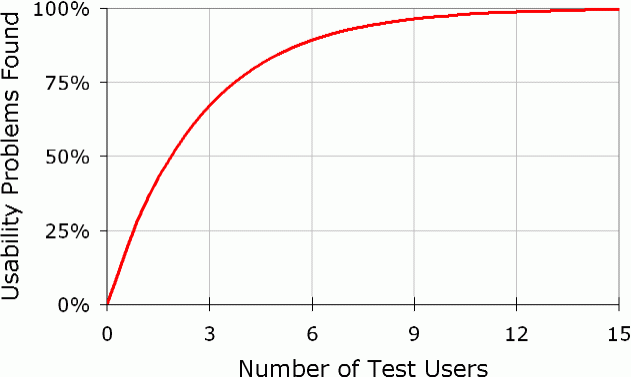
\includegraphics[width=250px]{img/nielsen2012_usertests}
	\end{center}
	\caption{The curve shows the user test's diminishing returns beyond a certain amount of test users; adapted from \url{http://www.nngroup.com/articles/why-you-only-need-to-test-with-5-users/}.}
	\label{fig:nielsengraph}
\end{figure}


\subsubsection{Usability engineering}

In \cite{duval:2012:chi:evaluation}, two methods are described to perform usability engineering tests: usability labs, and think aloud\index{think aloud} testing. In a usability lab the user is observed while performing certain tasks. Data on task completion time, mouse clicks, eye-movement can be collected. Direct observation or cameras can be used to observe the user. To mimic real-life situations, also complete settings can be recreated in which the users would normally use the application\cite{duval:2012:chi:evaluation}.

Using usability labs can be rather costly, as labs need to be available and the required equipment may be expensive. The think aloud protocol is a variation on the usability lab method and is cheaper to perform, cf. 'discount usability engineering'\cite{duval:2012:chi:evaluation}. During a think aloud test, the user describes his/her reasoning for each action he/she undertakes\cite{nielsen:2012:nngroup:think_aloud}. This method has several advantages and disadvantages, as listed in table \ref{table:usability_engineering}, based on \cite{nielsen:2012:nngroup:think_aloud} and \cite{snyder:2003}.


\begin{table}%
	\begin{center}
		\begin{tabular}{l p{300px}}
			\hline
			Advantages		&		It is cheap to perform; \\
										&		It is robust; \\
										&		It is flexible; \\
										&		It is convincing; \\
										&		It is easy to learn; \\
			\hline
			Disadvantages	&		It creates an unnatural situation, as users usually don't say out loud everything they are about to do or think; \\
										&		The user may tend to filter his/her statements to avoid saying things that he/she may find silly or uninteresting; \\
										&		The facilitator may introduce bias in user behavior if he/she provides too much information when answering or instructing users; \\
			\hline
		\end{tabular}
	\end{center}
	\caption{Advantages and disadvantages of the think aloud protocol.}
	\label{table:usability_engineering}
\end{table}

\subsubsection{Questionnaires}

To obtain information other than observational data, the user is presented with a summative questionnaire. Questionnaires are used to obtain subjective information from the user about the user's experiences. Table \ref{table:questionnaires} lists several advantages and disadvantages of the use of questionnaires in usability studies, based on \cite{kirakowski:2013}.

\begin{table}%
	\begin{center}
		\begin{tabular}{l p{300px}}
			\hline
			Advantages		&		Evaluates the point of view of the user; \\
										&		Measures gained from a questionnaire are to a large extent, independent of the system, users, or tasks to which the questionnaire was applied; \\
										&		Quick and cost effective; \\
			\hline
			Disadvantages	&		Only the user's reaction as the user perceives the situation; \\
										&		Lack of detail, as questionnaires are usually designed to fit a number of different situations; \\
										&		Subjective data must be enhanced with performance, mental effort, and effectiveness data. \\
			\hline
		\end{tabular}
	\end{center}
	\caption{Advantages and disadvantages of the questionnaires.}
	\label{table:questionnaires}
\end{table}


There are several standardized questionnaires. The one used for the application evaluation is the system usability scale\index{system usability scale} (SUS). A system usability scale test is a questionnaire that consists out of ten specific questions that attempts to measure the user's perception of the application's usability. Each question is answered by checking one out of five checkboxes: checkbox one corresponds to strong disagreement with the statement, the fifth checkbox corresponds to strong agreement with the statement\cite{sauro:2011}. The ten questions are listed in appendix \ref{appendix:sus}.


\section{Story board}


\section{Iteration 1: paper prototype}\label{chapter:prototype:section:paper}

% 6. testen...
%		+ doel: wat wil je te weten komen?
%		+ methode: hoe ga je dat te weten komen?
%		+ rationale: welke andere manieren heb je overwogen en waarom niet weerhouden?
%		+ wie, wat, waar: n, demographics, logistics, ...
%		+ resultaten: wat heb je gemeten, geobserveerd? (zonder interpretatie)
%		+ besluit: wat ben je te weten gekomen? (link naar resultaten)
% 7. itereren...
%		+ doel: belangrijkste proble(e)m(en) dat/die je wil aanpakken
%		+ alternatieven: hoe kan je problemen aanpakken
%		+ keuze: en rationale
%		+ herneem die problemen bij volgende iteratie!



\section{Iteration 2: first digital prototype (SoundSuggest 1.x)}\label{chapter:prototype:section:soundsuggest1}




\section{Iteration 3: second digital prototype (SoundSuggest 2.x)}\label{chapter:prototype:section:soundsuggest2}




\section{Iteration 4: third digital prototype (SoundSuggest 3.x)}\label{chapter:prototype:section:soundsuggest3}





